% !TeX root = ../../thesis.tex

For completeness, we used the inverse of the percentage of nulls in the training set. For plausibility, several methods were applied. The first was a Bayesian network. 

In our approach, Bayesian networks, which are probabilistic graphical models, play a pivotal role in predicting the plausibility of different elements. These networks are structured as directed acyclic graphs, where each node represents a variable and edges denote conditional dependencies among these variables \unskip~\cite{pearl1988probabilistic}. This structure allows the network to efficiently manage and represent the probabilistic relationships between multiple variables. The core strength of Bayesian networks in our context lies in their ability to predict the plausibility of various elements by analyzing these interdependencies. By integrating the conditional probabilities of variables and their dependencies, the network can infer the likelihood of certain outcomes or states, thereby assessing the plausibility of different columns in our dataset, when compared with the registered value. 

With this, we hope to capture the heterogeneous essence of the data, as well as possible outliers that are also plausible. We chose this model for its dual advantages: its capability to classify the plausibility of all columns within a single unified framework, and its interpretability, which allows for a clearer understanding of how each variable influences the overall plausibility prediction. The networks were created with the pgmpy package \unskip~\cite{pgmpy}. 

Secondly, we added the outlier-tree method\unskip~\cite{cortesExplainableOutlierDetection2020} which tries to integrate a decision tree that ''predicts'' the values of each column based on the values of each other column. In the process, every time separation is evaluated, it takes observations from each branch as a homogeneous cluster to search for outliers in the predicted 1-d distribution of the column. Outliers are determined according to confidence intervals in this 1-d distribution and need to have large gaps in order to be marked as outliers in the next observation. Because it looks for outliers in the branch of the decision tree, it knows the conditions that make it a rare observation relative to other observation types corresponding to the same conditions, and these conditions are always related to target variables (as predicted by them).  As such, it can only detect outliers described by decision tree logic, and unlike other methods such as isolation forests, it can not assign outlier points to each observation, or detect outliers that are generally rare, but will always provide human-readable justification when it recognizes outliers. Therefore, these methods not only identify anomalies based on a single column/variable but also consider the context of the data, providing a more nuanced understanding of what constitutes an outlier. This contextual awareness ensures that the outliers are not merely statistical deviations but are also substantively significant within the specific framework of the target variables. 

We added also elliptic envelope and Local Outlier Factor as complementary models to these two. Elliptic envelope is a method that assumes a Gaussian distribution of data, fitting an ellipse to the central data points to identify outliers. It works best with normally distributed data but is less effective in higher dimensions or non-normal distributions. Local Outlier Factor measures the local density deviation of a data point relative to its neighbors, identifying outliers without assuming a specific data distribution. It is versatile for different data structures but sensitive to parameter settings, like the number of neighbors. 

An Interquartile Range (IQR) based metric was also added as a supportive metric. This metric used the difference between Q1 and the triple of IQR  to define a lower threshold and Q3 + 3IQR to define an upper threshold. We only categorized as outlier the values that fell outside these margins. Finally, a rule system was implemented to leverage domain knowledge in the overall scoring. The system is based on great expectations package \unskip~\cite{GXProactiveCollaborative}. A set of 17 rules was defined by the team, focusing on impossible numbers or relationship between variables  or value format. The rules covered plausability and conformance. 

The Conformance-based were related to technical issues like the format of dates (date of birth like d/m/y), and conformance to the value set (i.e. Robson group, bishop scores, or delivery types). Plausibility rules were linked to expected values for BMI, weight, and gestational age (gestational age between 20 and 44). We also added plausibility for the relationship between columns, namely weight across different weeks of gestation (weight week 35 {\textgreater} weight week 25). We have also added a relationship of greatness between ultrasound weights more than 5 weeks apart. 

As for preprocessing, all null representations were standardized, we also removed features with high missing rates ({\textgreater} 80\% ). The imputation process was performed with the median for continuous and a new category (NULLIMP) for categorical variables.

For the usage of the Bayesian network in particular, the continuous variables were discretized into three bins defined by quantile. We defined three as the number of bins in order to reduce the number of states in each node of the network. The evaluation was done with cross-validation with 10 splits and two repetitions for each column as the target.

The API for serving the prediction models was developed with FastAPI. So, the methods applied in terms of the DQA framework shown in figure \ref{fig:categories} are described in the table \ref{tab:methods}.

\begin{table}[htpb]
\caption{Implemented Methods in the tool. The first column is the category or data quality dimension. The second is a subcategory of the first column if applicable and the third column is the actual method used to assess such a dimension.} \label{tab:methods}
\renewcommand{\arraystretch}{1.4}
\setlength{\tabcolsep}{10pt}

\begin{tabularx}{\textwidth}{ p{2cm} p{3.5cm} X }
\hline
 Category   & Subcategory           & Method   \\ \hline
Completeness     & N/A               & Score by the inverse percentage of missing in the train data         \\ 
Plausibility & Atemporal Plausibility & Bayesian model prediction based on the other values of row \\ 
Plausibility & Atemporal Plausibility         & Z-score for column value based on IQR train data       \\    
Plausibility & Atemporal Plausibility           & Elliptic Envelope                       \\ 
Plausibility & Atemporal Plausibility           & Local Outlier Factor                \\ 
Conformance & Value Conformance           & Manual Rule engine                           \\ 
Plausibility & Atemporal Plausibility           & Manual Rule engine                      \\ 
Plausibility & Atemporal Plausibility           & outlier-tree                      \\ 
Conformance & Value Conformance & Manual Rule engine\\
\hline
\end{tabularx}

\end{table}


For trying to compile all of these models into a single value, that could grasp the quality of the row or patient, a scoring method was created. The method of calculating the final score is stated in figure \ref{fig:scoring_method}. 
%TC:ignore
\begin{figure}[htbp]
    \centering
    \caption{Workflow and weights used for creating the final score and which elements are used to do so.}\label{fig:scoring_method} 
    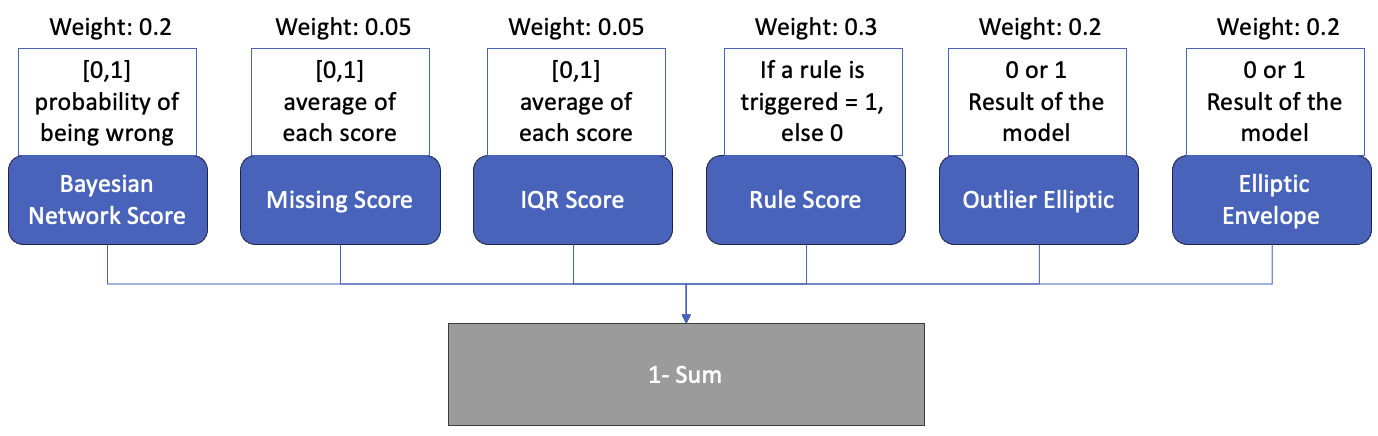
\includegraphics[scale=0.29]{figures/score-method.png}
    \end{figure}
    %TC:endignoregrama

To assess the tool's usefulness, we implemented it in a production environment and collect metrics regarding the data being produced. Then we presented some rows (or patient's records) to selected obstetrics clinicians for them to assess how likely the information is to be suitable for usage and rank it according to the perceived quality of the record. This was done through questionnaire, presenting the data and asking the clinicians to rank them from 1-10 and to describe the most important feature for the decision. We then compared the results with the ones from the model to make sanity checks regarding the model's performance and adequacy. We used Kendal Tau and Average Spearman's Rank Correlation Coefficient. Kendall Tau is a non-parametric statistic used to measure the strength and direction of the association between two ordinal variables. It calculates the difference between the number of concordant and discordant pairs of observations, normalized to ensure a value between -1 (perfect disagreement) and 1 (perfect agreement). Spearman's rank correlation coefficient is a non-parametric measure that assesses the strength and direction of a monotonic relationship between two ranked variables. It is based on the ranked values of the variables rather than their raw data, producing a value between -1 (perfect inverse relationship) and 1 (perfect direct relationship). Finally, we tested the capability of the model to discriminate bad quality records from good quality records, testing various thresholds of rank of quality, taken into account physicians responses.
We wrote all the code in Python 3.10.6 with the usage of the scikit-learn library for preprocessing, and evaluation\unskip~\cite{scikit-learn}.
